\chapter{Исследовательский инструментарий}\label{ch:ch3}

\section{Онтологизация предметной области}\label{sec:ch3/sect1}

\subsubsection{Тройной каскад}
В качестве необходимой модификации двойного каскада была предложена тройная каскадная схема, которая позволяет решить проблему возврата необходимого количества регенерата в цикл.
Такая схема представлена на рис. \ref{fig:triple}.
Здесь, первый каскад, как и на схеме рис. \ref{fig:double_ru}, увеличивает концентрацию $^{235}$U с сопутствующими легкими изотопами и направляет их во второй каскад.
В этом каскаде, также как и в предыдущей схеме, $^{232,234}$U концентрируются в потоке загрязненного продукта \cite{smirnovObogashchenieRegenerirovannogoUrana2018}.
Но на этот раз изотопный состав, полученный в тяжелой фракции не является конечным продуктом. 
Теперь он разбавляется предварительно подготовленным НОУ, изготовленным из природного урана.
Это необходимо по двум причинам:
\begin{enumerate}
  \item для контроля концентраций $^{232,234}$U в допустимых пределах.
  \item для управления соотношением питающего регенерата к финальному продукту, что обеспечивает поддержание требуемого уровня возврата регенерата в ЯТЦ.
\end{enumerate}

\begin{figure}[ht]
  \centerfloat{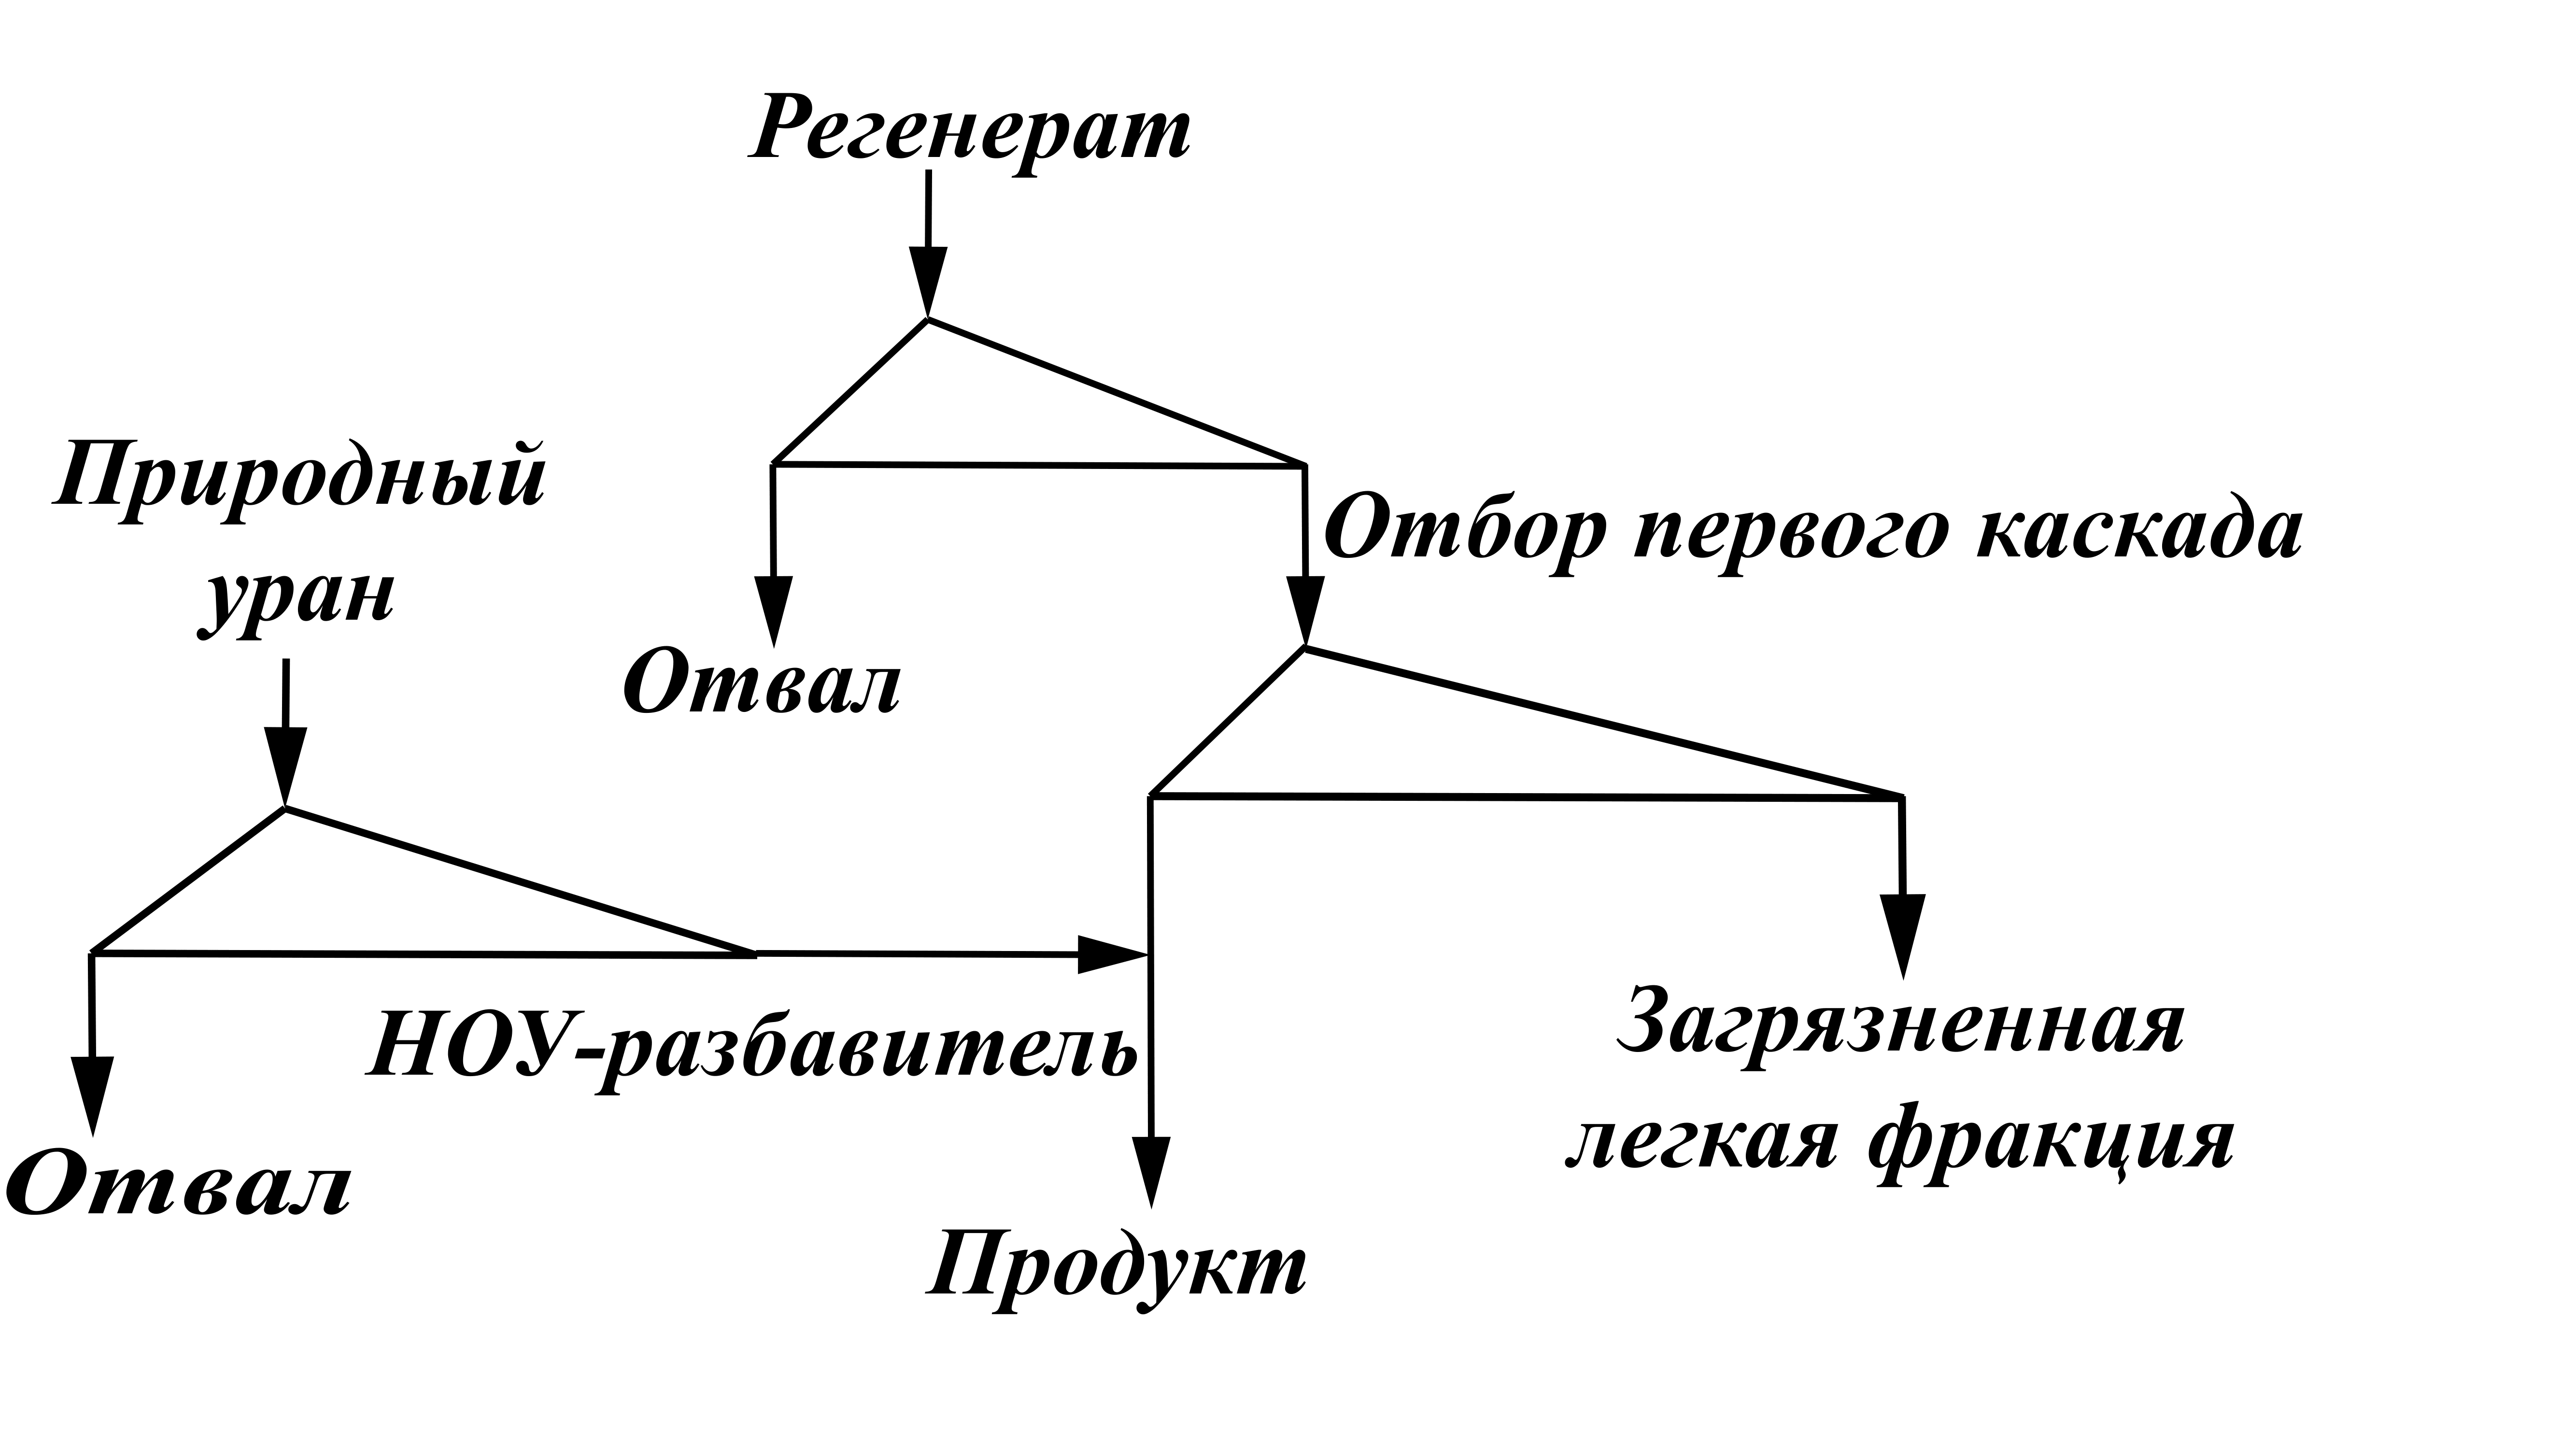
\includegraphics[scale=0.07]{cascades/triple}}
  \caption{Тройной каскад}\label{fig:triple}
\end{figure}

Хотя этот вариант и кажется идеальным, все еще остается нерешенной судьба легкой фракции второго каскада.



\clearpage